% IEEE Conference Template for ML/AI Papers
% Document class specification - conference format for IEEE
\documentclass[conference]{IEEEtran}

% Override command lockouts (typically needed for IEEE papers)
\IEEEoverridecommandlockouts
% The preceding line is only needed to identify funding in the first footnote. If that is unneeded, please comment it out.
\tracinglostchars=0

%%%%%%%%%%%%%%%%%%%%%%%%%%%%%%%%%%%%%%%%%
% PACKAGES
%%%%%%%%%%%%%%%%%%%%%%%%%%%%%%%%%%%%%%%%%
% Citation management
\usepackage{cite}                    % For bibliography citations

% Text and list formatting
\usepackage{enumitem}                % Enhanced list environments
\usepackage{amsmath,amssymb,amsfonts} % Mathematical symbols and fonts

% Algorithms
\usepackage{algorithm}               % For algorithm environments
\usepackage{algorithmic}             % For algorithm formatting

% Graphics and visual elements
\usepackage{graphicx}                % For including images
\usepackage{textcomp}                % Text companion fonts
\usepackage{xcolor}                  % For colored text
\usepackage{forest}                  % For drawing tree diagrams

% TikZ and related packages for diagrams
\usepackage{tikz}                    % Core package for creating graphics
\usepackage{adjustbox}               % For scaling figures
\usepackage{url}                     % For formatting URLs

% Figure and table enhancements
\usepackage{pgfplots}                % For creating plots
\usepackage{booktabs}                % For professional-looking tables
\usepackage{colortbl}                % For colored table cells
\pgfplotsset{compat=1.18}

% TikZ libraries for specific diagram types
\usetikzlibrary{shapes.geometric,arrows,positioning,fit,backgrounds,calc,decorations.pathreplacing,decorations.markings,patterns,circuits.logic.US,matrix,chains}

% Table enhancements
\usepackage{threeparttable}          % For table notes
\usepackage{cuted}                   % For multi-column environments

% Custom command for line breaks in author block
\makeatletter
\newcommand{\linebreakand}{%
  \end{@IEEEauthorhalign}
  \hfill\mbox{}\par
  \mbox{}\hfill\begin{@IEEEauthorhalign}
}
\makeatother

% Define custom colors for visualizations
% These are common colors used in AI/ML papers
\definecolor{qubitblue}{RGB}{70,130,180}      % Blue for primary elements
\definecolor{controlred}{RGB}{220,20,60}      % Red for control elements
\definecolor{aigreen}{RGB}{50,150,50}         % Green for AI components
\definecolor{quantumpurple}{RGB}{128,0,128}   % Purple for quantum elements
\definecolor{errororange}{RGB}{255,140,0}     % Orange for error highlighting
\AddToHook{env/thebibliography/begin}{\label{ReferencesStart}}

%%%%%%%%%%%%%%%%%%%%%%%%%%%%%%%%%%%%%%%%%
% DOCUMENT BEGINS
%%%%%%%%%%%%%%%%%%%%%%%%%%%%%%%%%%%%%%%%%
\begin{document}
\raggedbottom

%%%%%%%%%%%%%%%%%%%%%%%%%%%%%%%%%%%%%%%%%
% TITLE SECTION
%%%%%%%%%%%%%%%%%%%%%%%%%%%%%%%%%%%%%%%%%
\title{Spatiotemporal Generative Models for Video and 4D Scenes: Architectures, Control, and Evaluation}

\author{
    \IEEEauthorblockN{Author Name(s) TBD}
    \IEEEauthorblockA{Affiliation(s) TBD\\Email(s) TBD}
}

\maketitle

%%%%%%%%%%%%%%%%%%%%%%%%%%%%%%%%%%%%%%%%%
% KEYWORDS
%%%%%%%%%%%%%%%%%%%%%%%%%%%%%%%%%%%%%%%%%
\begin{IEEEkeywords}
spatiotemporal generative models, video generation, text-to-video, world simulators, temporal coherence, motion control, physics-aware generation, 4D scenes, Gaussian splatting
\end{IEEEkeywords}

%%%%%%%%%%%%%%%%%%%%%%%%%%%%%%%%%%%%%%%%%
% ABSTRACT
%%%%%%%%%%%%%%%%%%%%%%%%%%%%%%%%%%%%%%%%%
\begin{abstract}
Spatiotemporal generative models have advanced from short, stylized clips to systems that can synthesize longer videos, follow structured motion controls, and, in some settings, support interactive rollouts.
In parallel, a fast-growing line of work generates explicit 3D/4D scene representations (e.g., dynamic radiance fields and Gaussian splats) that enable re-rendering under viewpoint changes and more direct scene editing.
This review surveys objectives and architectures for video and 4D generation, with an emphasis on temporal coherence, motion/camera control, and the role of physics and interaction priors.
We propose a control-surface view that unifies prompting, trajectory/camera interfaces, and editing operators, summarize evidence regimes for frontier systems, and recommend evaluation protocols that stress-test coherence, controllability, and geometric consistency beyond average-case realism.
Our goal is a practical, evidence-bounded map of design choices and evaluation practices for researchers and practitioners building video ``world simulators'' and 4D generative pipelines.
\end{abstract}

%%%%%%%%%%%%%%%%%%%%%%%%%%%%%%%%%%%%%%%%%
% INTRODUCTION
%%%%%%%%%%%%%%%%%%%%%%%%%%%%%%%%%%%%%%%%%
\section{Introduction and Scope}
Recent progress in generative modeling has turned video from a niche output modality into a scalable target for large spatiotemporal generators.
Diffusion-based video models demonstrate strong perceptual quality and text alignment, and have become a common backbone for both research prototypes and deployed systems \cite{ho2020denoising,ho2022video,ho2022imagen,blattmann2023stable,bartal2024lumiere}.
At the same time, token-based and hybrid approaches explore alternative training and control interfaces, blurring lines between ``video generation'' and broader sequence modeling \cite{villegas2022phenaki,kondratyuk2023videopoet,polyak2024movie}.

Beyond short clips, a recurring aspiration is to treat a generator as a controllable simulator: a model that maintains persistent scene state, responds to interventions, and supports interactive rollouts.
This framing appears explicitly in recent technical reports and in research on generative interactive environments \cite{openai2024worldsimulators,bruce2024genie,savov2025exploration}.
In practice, the ``world simulator'' label spans a spectrum of task settings, from open-loop text-to-video to closed-loop environment generation for agent interaction \cite{bruce2024genie,savov2025exploration,yang2025geniedrive}.

This review focuses on three tightly coupled themes:
(i) video models as scalable spatiotemporal generators (and when such models meaningfully support ``world simulator'' claims),
(ii) temporal coherence, motion control, and physics/interaction priors, and
(iii) 3D/4D-aware generation and rendering, where the output is a dynamic scene representation rather than pixels alone \cite{mildenhall2020nerf,kerbl20233d,wu20234d}.
We emphasize evidence-bounded comparisons, control interfaces, and evaluation protocols, while avoiding repetitive year-centric narration.
Figure~\ref{fig:task-map} summarizes the task settings and evaluation axes used throughout the paper.

\begin{figure}[t]
    \centering
    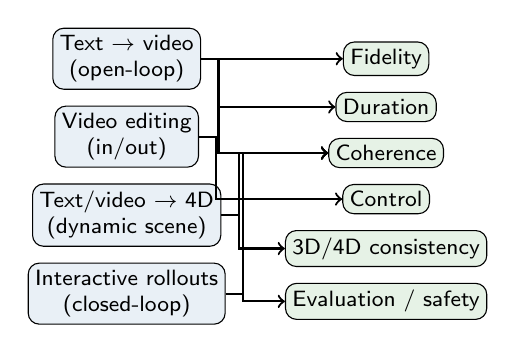
\begin{tikzpicture}[
        node distance=2mm,
        font=\sffamily\footnotesize,
        task/.style={rectangle, rounded corners, draw, fill=qubitblue!12, inner sep=2.5pt, align=center},
        axis/.style={rectangle, rounded corners, draw, fill=aigreen!12, inner sep=2.5pt, align=center},
        arrow/.style={->, thick}
    ]
        \node[task] (t2v) {Text $\rightarrow$ video\\(open-loop)};
        \node[task, below=of t2v] (edit) {Video editing\\(in/out)};
        \node[task, below=of edit] (t24d) {Text/video $\rightarrow$ 4D\\(dynamic scene)};
        \node[task, below=of t24d] (loop) {Interactive rollouts\\(closed-loop)};

        \node[axis, right=1.8cm of t2v] (ax1) {Fidelity};
        \node[axis, below=of ax1] (ax2) {Duration};
        \node[axis, below=of ax2] (ax3) {Coherence};
        \node[axis, below=of ax3] (ax4) {Control};
        \node[axis, below=of ax4] (ax5) {3D/4D consistency};
        \node[axis, below=of ax5] (ax6) {Evaluation / safety};

        \foreach \src in {t2v,edit,t24d,loop} {
            \draw[arrow] (\src.east) -- ++(0.22,0) |- (ax3.west);
        }
        \draw[arrow] (t2v.east) -- ++(0.22,0) |- (ax1.west);
        \draw[arrow] (t2v.east) -- ++(0.22,0) |- (ax2.west);
        \draw[arrow] (edit.east) -- ++(0.22,0) |- (ax4.west);
        \draw[arrow] (t24d.east) -- ++(0.22,0) |- (ax5.west);
        \draw[arrow] (loop.east) -- ++(0.22,0) |- (ax6.west);
    \end{tikzpicture}
    \caption{Task settings and evaluation axes used throughout the paper. We treat ``world simulator'' claims as a spectrum, and separate open-loop generation from closed-loop interactive rollouts \cite{openai2024worldsimulators,bruce2024genie,savov2025exploration}.}
    \label{fig:task-map}
\end{figure}

Our contributions are:
\begin{itemize}[leftmargin=*]
    \item a compact taxonomy of spatiotemporal generative objectives, representations, and spacetime backbones \cite{ho2022video,lipman2022flow,liu2022flow};
    \item a control-surface view of coherence mechanisms and motion/camera interfaces for generation and editing \cite{guo2023animatediff,wang2023motionctrl,liu2023video,wang2025bullettime};
    \item a 3D/4D-aware perspective that connects video generators to dynamic scene representations and rendering-time constraints \cite{mildenhall2020nerf,kerbl20233d,wu20234d,xu20254dgt};
    \item practical evaluation guidance, highlighting what common metrics capture and where they fail \cite{unterthiner2018towards,huang2023vbench,sun2024t2v,mou2025gradeo}.
\end{itemize}

%%%%%%%%%%%%%%%%%%%%%%%%%%%%%%%%%%%%%%%%%
% BACKGROUND
%%%%%%%%%%%%%%%%%%%%%%%%%%%%%%%%%%%%%%%%%
\section{Foundations: Spatiotemporal Generative Modeling}
We organize spatiotemporal generators along three axes: (i) the \emph{generative objective} (diffusion/score vs transport/flow vs autoregressive), (ii) the \emph{representation} (pixels, latents, or tokens), and (iii) the \emph{output type} (video frames vs 3D/4D scene representations).
This section introduces these building blocks and the design tradeoffs they induce \cite{ho2020denoising,song2020score,lipman2022flow,liu2022flow}.
Figure~\ref{fig:taxonomy} provides a minimal taxonomy, and Figure~\ref{fig:backbone} sketches a backbone-level view of diffusion/flow-style generators \cite{ho2022video,bartal2024lumiere,wang2023motionctrl}.
Table~\ref{tab:objective-families} complements this view with a compact summary of objective families and their typical sampling profiles.

\subsection{Objectives: diffusion, score models, and transport}
Diffusion models learn to reverse a forward noising process, typically by predicting noise or a related target at multiple noise levels \cite{ho2020denoising}.
The continuous-time view unifies many variants under stochastic differential equations (SDEs) and clarifies the role of samplers and noise schedules \cite{song2020score}.
In parallel, transport-based objectives such as flow matching learn velocity fields that map a simple source distribution to the data distribution \cite{lipman2022flow}, and rectified-flow-style training seeks straighter trajectories that can reduce sampling cost \cite{liu2022flow}.
For video, these objectives interact with temporal consistency because sampling proceeds along a trajectory in model time while the generated content must remain coherent along \emph{scene time}.

\subsection{Representations: pixels, latents, and tokens}
Video generation is often memory-bound; many practical systems therefore operate in a learned latent space, amortizing high-resolution synthesis while retaining perceptual detail \cite{rombach2021high,blattmann2023stable}.
Tokenization offers an alternative that can support long-horizon modeling and discrete control interfaces, at the cost of representation bottlenecks and token design choices \cite{villegas2022phenaki,kondratyuk2023videopoet}.
For 3D/4D-aware generation, the representation may be an explicit scene model (e.g., Gaussians) that enables fast rendering and view-dependent effects, shifting some difficulty from generation to representation learning and optimization \cite{kerbl20233d,wu20234d,xu20254dgt}.

\subsection{Backbones: spacetime U-Nets and diffusion transformers}
Early video diffusion work often adapts image U-Nets by adding temporal convolutions or attention, balancing capacity against the quadratic cost of global spacetime attention \cite{ho2022video}.
Space-time diffusion designs model space and time jointly to improve coherence, while remaining compatible with diffusion training and guidance \cite{bartal2024lumiere}.
More recently, transformer backbones have become common in large generators, motivated by scaling behavior and unified token processing over space-time \cite{peebles2022scalable,polyak2024movie}.

\subsection{Conditioning and control channels}
Conditioning choices determine what the model can be \emph{asked} to do at inference time.
Text-to-video systems commonly use cross-attention to text embeddings, while additional controls (depth/pose/edges/trajectories) can be injected via dedicated control networks or adapters \cite{zhang2023adding,guo2023animatediff,wang2023motionctrl}.
Because control signals are often imperfect or underspecified, robustness to control noise and explicit mechanisms for temporal stabilization are central to long-horizon generation \cite{li2024enhancing,wang2025bullettime}.

\subsection{Scaling, factorization, and long-horizon generation}
Scaling video models stresses both training (data, compute, memory) and inference (sampling cost, temporal drift).
Recent systems therefore explore factorization strategies that decouple \emph{scene construction} from \emph{temporal synthesis}, aiming to preserve global consistency while extending duration \cite{hassan2025factorized,zhang2025endless}.
Autoregressive spacetime modeling provides another route to long-context generation, though it inherits tokenization and compounding-error challenges \cite{villegas2022phenaki,liu2025infinitystar,kondratyuk2023videopoet}.
Geometry-aware priors can further stabilize long rollouts by propagating 3D structure or by conditioning on intermediate scene state \cite{kong2025worldwarp,zhu2025astra}.

\begin{table}[t]
    \centering
    \renewcommand{\arraystretch}{1.05}
    \setlength{\tabcolsep}{4pt}
    \begin{tabular}{p{1.35cm} p{2.05cm} p{3.95cm}}
        \toprule
        Family & Sampling profile & Typical tradeoffs in video \\
        \midrule
        Diffusion / score & many-step denoising & strong quality; expensive sampling; needs explicit coherence mechanisms \cite{ho2020denoising,ho2022video} \\
        Flow matching / rectified & ODE/velocity fields & fewer-step generation possible; training/objective choices matter for stability \cite{lipman2022flow,liu2022flow} \\
        Auto-regressive tokens & token-by-token rollout & long context and discrete controls; sensitive to tokenization and error accumulation \cite{villegas2022phenaki,kondratyuk2023videopoet} \\
        \bottomrule
    \end{tabular}
    \caption{Objective families and their typical sampling profiles in spatiotemporal generation. Many practical systems hybridize these choices.}
    \label{tab:objective-families}
\end{table}

\begin{figure}[t]
    \centering
    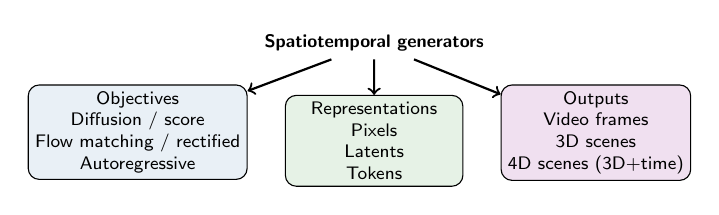
\begin{tikzpicture}[
        scale=0.82, transform shape,
        node distance=0.55cm,
        font=\sffamily\footnotesize,
        box/.style={rectangle, rounded corners, draw, fill=#1!12, align=center, inner sep=3pt, minimum width=2.75cm},
        title/.style={font=\sffamily\footnotesize\bfseries}
    ]
        \node[title] (h0) {Spatiotemporal generators};

        \node[box=qubitblue, below left=of h0, xshift=0.25cm] (obj) {Objectives\\Diffusion / score\\Flow matching / rectified\\Autoregressive};
        \node[box=aigreen, below=of h0] (rep) {Representations\\Pixels\\Latents\\Tokens};
        \node[box=quantumpurple, below right=of h0, xshift=-0.25cm] (out) {Outputs\\Video frames\\3D scenes\\4D scenes (3D+time)};

        \draw[->, thick] (h0) -- (obj);
        \draw[->, thick] (h0) -- (rep);
        \draw[->, thick] (h0) -- (out);
    \end{tikzpicture}
    \caption{A minimal taxonomy for video and 4D generators: objective family, representation, and output type. Concrete systems choose points in this space (often hybridizing choices) \cite{ho2022video,rombach2021high,lipman2022flow,kondratyuk2023videopoet,kerbl20233d,wu20234d}.}
    \label{fig:taxonomy}
\end{figure}

\begin{figure}[t]
    \centering
    \begin{adjustbox}{max width=\columnwidth}
    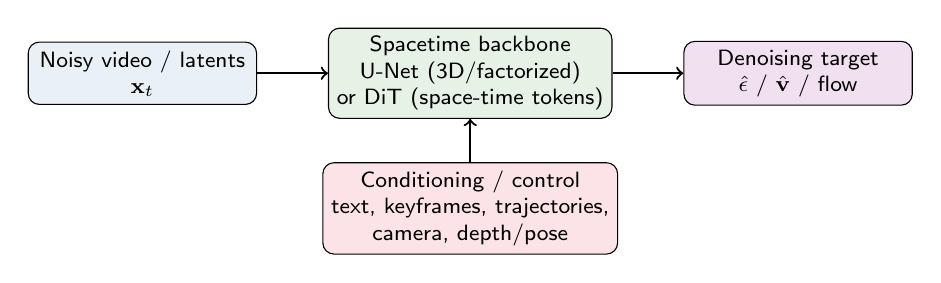
\begin{tikzpicture}[
        scale=1.0, transform shape,
        font=\sffamily\footnotesize,
        block/.style={rectangle, rounded corners, draw, fill=#1!12, inner sep=3pt, align=center, minimum width=2.9cm},
        arrow/.style={->, thick}
    ]
        \node[block=qubitblue] (x) {Noisy video / latents\\$\mathbf{x}_t$};
        \node[block=aigreen, right=0.9cm of x] (backbone) {Spacetime backbone\\U-Net (3D/factorized)\\or DiT (space-time tokens)};
        \node[block=quantumpurple, right=0.9cm of backbone] (eps) {Denoising target\\$\hat{\epsilon}$ / $\hat{\mathbf{v}}$ / flow};

        \draw[arrow] (x) -- (backbone);
        \draw[arrow] (backbone) -- (eps);

        \node[block=controlred, below=0.55cm of backbone, minimum width=3.0cm] (cond) {Conditioning / control\\text, keyframes, trajectories,\\camera, depth/pose};
        \draw[arrow] (cond.north) -- (backbone.south);
    \end{tikzpicture}
    \end{adjustbox}
    \caption{Backbone schematic for diffusion/flow generators with conditioning controls.}
    \label{fig:backbone}
\end{figure}

%%%%%%%%%%%%%%%%%%%%%%%%%%%%%%%%%%%%%%%%%
% BUILDING BLOCKS / TAXONOMY
%%%%%%%%%%%%%%%%%%%%%%%%%%%%%%%%%%%%%%%%%
\section{Frontier Systems and World-Simulator Framing}
Frontier video generators span a wide range of disclosure regimes.
Some are released as detailed technical reports (often on arXiv) with explicit evaluation sections \cite{bartal2024lumiere,polyak2024movie,bruce2024genie}, while others are primarily described via product documentation, system cards, or API references \cite{openai2024worldsimulators,openai2024sorasystemcard,openai2025sora2,googlecloud2025veomodelapi,runway2025gen45,luma2025ray3}.
This creates a fundamental asymmetry: closed systems may expose rich user-facing controls, but provide limited information about training data, compute, and standardized evaluation protocols \cite{openai2024sorasystemcard,googlecloud2025veomodelapi}.

\subsection{Capability axes and evidence types}
We compare systems along axes that matter for downstream use and scientific evaluation: perceptual fidelity, duration, temporal coherence, controllability, and (when applicable) geometric/3D consistency.
For each axis, we treat the \emph{evidence type} as part of the claim: peer-reviewed or arXiv reports (stronger for measurable attributes), official docs/system cards (stronger for availability and documented controls), and third-party anecdotes (excluded from quantitative comparison).
When a field is not explicitly disclosed, we mark it as unknown rather than inferring it \cite{openai2024sorasystemcard,googlecloud2025veomodelapi}.

\subsection{A compact comparison snapshot}
Table~\ref{tab:system-compare} summarizes a small set of representative systems and what can be reliably said about them from public sources.
The goal is not a leaderboard; it is a transparency-aware map of what claims are \emph{supported} and what remains underspecified \cite{openai2024sorasystemcard,googlecloud2025veomodelapi,runway2025gen45}.
Figure~\ref{fig:timeline} provides an illustrative (non-exhaustive) timeline of a few widely cited milestones and documented releases.

\begin{figure}[t]
    \centering
    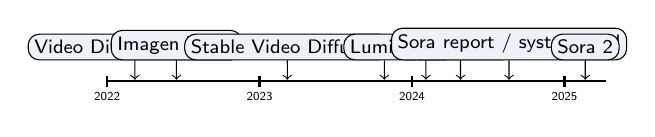
\begin{tikzpicture}[
        scale=0.88, transform shape,
        font=\sffamily\footnotesize,
        event/.style={rectangle, rounded corners, draw, fill=qubitblue!10, inner sep=2.5pt, align=left},
        tick/.style={draw, thick},
        lab/.style={font=\sffamily\tiny}
    ]
        \draw[tick] (0,0) -- (7.2,0);
        \foreach \x/\y in {0/2022,2.2/2023,4.4/2024,6.6/2025} {
            \draw[tick] (\x,0.08) -- (\x,-0.08);
            \node[lab] at (\x,-0.22) {\y};
        }

        \node[event, above=3mm of {(0.4,0)}] (vdm) {Video Diffusion Models};
        \node[event, above=3mm of {(1.0,0)}] (imagenv) {Imagen Video};
        \node[event, above=3mm of {(2.6,0)}] (svd) {Stable Video Diffusion};
        \node[event, above=3mm of {(4.0,0)}] (lumiere) {Lumiere};
        \node[event, above=3mm of {(4.6,0)}] (genie) {Genie};
        \node[event, above=3mm of {(5.1,0)}] (moviegen) {Movie Gen};
        \node[event, above=3mm of {(5.8,0)}] (sora) {Sora report / system card};
        \node[event, above=3mm of {(6.9,0)}] (sora2) {Sora 2};

        \draw[->] (vdm.south) -- (0.4,0.02);
        \draw[->] (imagenv.south) -- (1.0,0.02);
        \draw[->] (svd.south) -- (2.6,0.02);
        \draw[->] (lumiere.south) -- (4.0,0.02);
        \draw[->] (genie.south) -- (4.6,0.02);
        \draw[->] (moviegen.south) -- (5.1,0.02);
        \draw[->] (sora.south) -- (5.8,0.02);
        \draw[->] (sora2.south) -- (6.9,0.02);
    \end{tikzpicture}
    \caption{Illustrative timeline of a few widely cited milestones and publicly documented releases (not exhaustive). Each label corresponds to a specific public report or documentation source \cite{ho2022video,ho2022imagen,blattmann2023stable,bartal2024lumiere,bruce2024genie,polyak2024movie,openai2024worldsimulators,openai2024sorasystemcard,openai2025sora2}.}
    \label{fig:timeline}
\end{figure}

\begin{table*}[t]
    \centering
    \renewcommand{\arraystretch}{1.05}
    \setlength{\tabcolsep}{4pt}
    \begin{threeparttable}
    \begin{tabular}{p{2.3cm} p{1.6cm} p{2.0cm} p{4.2cm} p{5.1cm}}
        \toprule
        System & Access & Output & Documented control surfaces & Public evidence (non-exhaustive) \\
        \midrule
        Sora / Sora 2 & Product & Video & Prompt + product/UI controls (details vary); safety disclosures\tnote{a} & OpenAI report + system card + release notes \cite{openai2024worldsimulators,openai2024sorasystemcard,openai2025sora2} \\
        Veo (Vertex AI) & API / cloud & Video & Prompt; API-level options; model/version-specific constraints\tnote{b} & Google Cloud model + API docs \cite{googlecloud2025veomodelapi,googlecloud2025veo2,googlecloud2025veo3} \\
        Runway Gen-4.5 & Product & Video & Prompt + documented creation workflow; product constraints\tnote{c} & Runway help docs \cite{runway2025gen45} \\
        Luma Ray3 & Product & Video & Prompt + product controls (undisclosed details in many cases) & Luma press/product page \cite{luma2025ray3} \\
        Pika (1.0+) & Product & Video & Prompt + product controls (undisclosed details in many cases) & Pika blog (milestones) \cite{pika2024raises80m} \\
        Stable Video Diffusion & Open weights & Video & Prompt + image/video conditioning (method dependent) & Open arXiv report with released weights \cite{blattmann2023stable} \\
        Lumiere / Movie Gen / Genie & Research reports & Video / environments & As reported in each paper (e.g., prompting, structured controls) & Technical reports and evaluations \cite{bartal2024lumiere,polyak2024movie,bruce2024genie} \\
        \bottomrule
    \end{tabular}
    \begin{tablenotes}[flushleft]
        \footnotesize
        \item[a] We treat system cards as evidence for safety/evaluation process, not as a complete specification of model internals.
        \item[b] Documented constraints vary by model version; use the cited docs for up-to-date API-facing details.
        \item[c] Product documentation is used for workflow and constraints; undisclosed fields are treated as unknown.
    \end{tablenotes}
    \end{threeparttable}
    \caption{Transparency-aware comparison: only fields explicitly supported by public sources are included; missing information is treated as unknown.}
    \label{tab:system-compare}
\end{table*}

\subsection{Reporting checklist for comparability}
For the community to evaluate ``world simulator'' progress without over-indexing on isolated demos, reports should make a small set of choices explicit: prompt sets, sampling settings, control inputs, and what is being measured.
Benchmark suites provide partial standardization but cannot replace transparent reporting \cite{huang2023vbench,unterthiner2018towards}.
We recommend a lightweight checklist (Table~\ref{tab:reporting-checklist}) that applies to both open papers and product-facing documentation.

\begin{table}[t]
    \centering
    \renewcommand{\arraystretch}{1.05}
    \setlength{\tabcolsep}{4pt}
    \begin{tabular}{p{1.55cm} p{5.7cm}}
        \toprule
        Item & What to disclose (minimum) \\
        \midrule
        Prompts & prompt sets, constraints, and any prompt filtering \cite{huang2023vbench} \\
        Sampling & steps, guidance, windowing/anchoring, post-processing \cite{li2024enhancing} \\
        Controls & which control surfaces are supported and failure modes under noisy controls \cite{wang2023motionctrl} \\
        Geometry & whether 3D/4D priors are used (explicit or implicit) \cite{kong2025worldwarp,gu2025diffusion} \\
        Safety & threat model, mitigations, and evaluation methods \cite{openai2024sorasystemcard} \\
        \bottomrule
    \end{tabular}
    \caption{A minimal reporting checklist for reproducible comparisons. When fields are undisclosed, downstream comparisons should treat them as unknown rather than inferred.}
    \label{tab:reporting-checklist}
\end{table}

Finally, we note a growing set of research systems that explicitly target long-horizon and interactive behavior, including 3D-aware long-video generation and general interactive world models \cite{zhang2025endless,zhu2025astra}.
These systems motivate evaluation beyond short clips and toward closed-loop consistency tests.

%%%%%%%%%%%%%%%%%%%%%%%%%%%%%%%%%%%%%%%%%
% FIGURES & DIAGRAMS
%%%%%%%%%%%%%%%%%%%%%%%%%%%%%%%%%%%%%%%%%

%%%%%%%%%%%%%%%%%%%%%%%%%%%%%%%%%%%%%%%%%
% FRONTIER MODELS / SYSTEMS
%%%%%%%%%%%%%%%%%%%%%%%%%%%%%%%%%%%%%%%%%
\section{Temporal Coherence and Motion Control}
Temporal coherence is the core bottleneck for treating a video generator as a reliable spatiotemporal engine.
Common failure modes include flicker, identity drift, inconsistent geometry across frames, and camera-motion artifacts; these failures often appear even when per-frame quality is high \cite{ho2022video,bartal2024lumiere,huang2023vbench}.
We summarize coherence mechanisms and control interfaces through a ``control surface'' lens: what inputs can the user (or an upstream planner) provide, and what consistency guarantees are empirically supported.

\subsection{Mechanisms for temporal consistency}
Coherence can be improved at multiple levels.
\emph{Architecture-level} mechanisms increase temporal receptive field (e.g., spacetime attention) but must manage quadratic complexity and memory \cite{ho2022video,bartal2024lumiere}.
\emph{Training-level} mechanisms introduce explicit temporal constraints (e.g., multi-frame supervision or structured motion priors), often trading flexibility for stability \cite{guo2023animatediff,wang2023motionctrl}.
\emph{Inference-level} mechanisms stabilize long generation through sliding windows, anchoring, or consistency post-processing without retraining, which is attractive for frontier or closed models where weights are inaccessible \cite{li2024enhancing}.
Figure~\ref{fig:coherence-matrix} sketches this design space.

\begin{figure}[t]
    \centering
    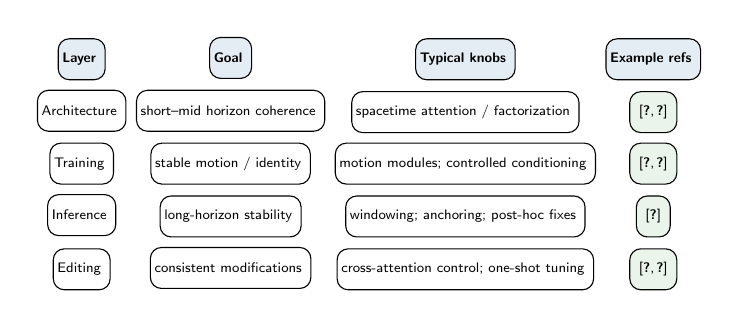
\begin{tikzpicture}[
        scale=0.83, transform shape,
        font=\sffamily\tiny,
        m/.style={matrix of nodes, nodes={draw, rounded corners, align=center, minimum height=5.2mm, inner sep=1.5pt}, column sep=1.2mm, row sep=1.2mm},
        h/.style={fill=qubitblue!14, font=\sffamily\tiny\bfseries},
        cell/.style={fill=white},
        ex/.style={fill=aigreen!10}
    ]
        \matrix[m] (mat) {
            |[h]| Layer & |[h]| Goal & |[h]| Typical knobs & |[h]| Example refs \\
            |[cell]| Architecture & |[cell]| short--mid horizon coherence & |[cell]| spacetime attention / factorization & |[ex]| \cite{ho2022video,bartal2024lumiere} \\
            |[cell]| Training & |[cell]| stable motion / identity & |[cell]| motion modules; controlled conditioning & |[ex]| \cite{guo2023animatediff,wang2023motionctrl} \\
            |[cell]| Inference & |[cell]| long-horizon stability & |[cell]| windowing; anchoring; post-hoc fixes & |[ex]| \cite{li2024enhancing} \\
            |[cell]| Editing & |[cell]| consistent modifications & |[cell]| cross-attention control; one-shot tuning & |[ex]| \cite{liu2023video,wu2022tune} \\
        };
    \end{tikzpicture}
    \caption{Coherence mechanisms by intervention layer. In practice, long-horizon stability often relies on inference-time strategies, while fine-grained edits commonly operate through attention control or targeted tuning \cite{liu2023video,li2024enhancing}.}
    \label{fig:coherence-matrix}
\end{figure}

\subsection{Control surfaces: from prompts to trajectories and cameras}
Control mechanisms can be grouped by the \emph{structure} of the provided constraint \cite{zhang2023adding,guo2023animatediff}.
Low-bandwidth controls include prompts and style references; higher-bandwidth controls specify spatial layouts, keyframes, object motion trajectories, or camera motion.
Control networks originally developed for images (e.g., ControlNet) motivate analogous interfaces for video, but temporal consistency makes the mapping nontrivial \cite{zhang2023adding,guo2023animatediff}.

Trajectory and camera controls are particularly important for world-simulator use cases because they provide an explicit handle on motion and viewpoint.
Representative approaches include unified motion controllers, tuning-free trajectory control, and explicit disentanglement between camera pose and temporal progression \cite{wang2023motionctrl,qiu2024freetraj,wang2025bullettime}.
Zero-shot object motion control is another complementary direction, aiming to steer moving entities without task-specific finetuning \cite{chen2024motion}.
Camera control can also be framed as an editing task on user-provided videos \cite{zhang2024recapture}.
Related ``re-angle'' formulations cast viewpoint changes as video-to-video translation with implicit 4D structure \cite{jeong2025reangle}.
Figure~\ref{fig:control-taxonomy} summarizes common control surfaces.
Table~\ref{tab:control-methods} provides a concrete mapping from control surfaces to representative methods (not exhaustive).

\begin{table*}[t]
    \centering
    \renewcommand{\arraystretch}{1.05}
    \setlength{\tabcolsep}{4pt}
    \begin{tabular}{p{2.2cm} p{3.4cm} p{4.2cm} p{6.1cm}}
        \toprule
        Control surface & Typical signal & Representative methods & Notes / failure modes \\
        \midrule
        Motion adapters & learned temporal modules & AnimateDiff \cite{guo2023animatediff} & Reuses image priors; can drift for long horizons without stabilization. \\
        Trajectories & sparse paths / keypoints & MotionCtrl, FreeTraj \cite{wang2023motionctrl,qiu2024freetraj} & Sensitive to underspecified depth/occlusion; may trade fidelity for control adherence. \\
        Camera & pose/path/time & BulletTime, ReCapture \cite{wang2025bullettime,zhang2024recapture} & Camera control can conflict with identity/persistence unless geometry or anchors are used. \\
        Zero-shot motion & object motion edits & Motion-Zero \cite{chen2024motion} & Control success depends on object segmentation/association and prompt ambiguity. \\
        Attention edits & cross-attention control & Video-P2P \cite{liu2023video} & Good for localized semantic edits; can break global motion consistency. \\
        One-shot tuning & video-specific finetune & Tune-A-Video \cite{wu2022tune} & Preserves a specific video style/identity; limited transfer across scenes. \\
        Region constraints & in-context spatial edits & Region-Constraint editing \cite{zhang2025region} & Strong locality; needs temporal stabilization to prevent flicker at boundaries. \\
        Structure distillation & tracking-derived motion & Structure From Tracking \cite{fei2025structure} & Improves motion structure; depends on tracker quality and domain shift. \\
        \bottomrule
    \end{tabular}
    \caption{Control surfaces and representative methods. The table is illustrative; many systems combine multiple controls and add inference-time stabilization \cite{li2024enhancing}.}
    \label{tab:control-methods}
\end{table*}

\begin{figure}[t]
    \centering
    \begin{adjustbox}{width=\columnwidth}
    \begin{forest}
    for tree={
        draw,
        rounded corners,
        align=left,
        font=\sffamily\tiny,
        s sep=1.3mm,
        l sep=2.2mm,
        edge={->, thick},
        fill=qubitblue!8,
    }
    [Control surfaces
        [Prompt / reference
            [text prompt]
            [style / image prompt]
        ]
        [Spatial / semantic
            [masks / regions]
            [edges / depth / pose]
        ]
        [Temporal / motion
            [keyframes]
            [object trajectories]
        ]
        [Camera
            [camera path / pose]
            [time--camera disentanglement]
        ]
        [Editing operators
            [cross-attention control]
            [one-shot tuning]
        ]
    ]
    \end{forest}
    \end{adjustbox}
    \caption{A control-surface taxonomy for video generation and editing. Different methods expose different subsets of these interfaces, with varying robustness to underspecified or noisy controls \cite{zhang2023adding,guo2023animatediff,wang2023motionctrl,liu2023video,wu2022tune,wang2025bullettime}.}
    \label{fig:control-taxonomy}
\end{figure}

\subsection{Long-horizon and multi-shot coherence}
Long-horizon generation amplifies small inconsistencies into visible drift: character identity changes, object persistence failures, and camera-motion artifacts accumulate across windows \cite{li2024enhancing,huang2023vbench}.
A common mitigation is to introduce hierarchical or multistage generation, where a coarse plan (scene layout, keyframes, or motion scaffold) is refined into higher-frequency details, reducing the burden on a single denoising trajectory \cite{hassan2025factorized,jain2025lights}.
Another perspective is to make structure explicit: tracking- or correspondence-derived signals can distill structure-preserving motion cues that improve stability under edits and long rollouts \cite{fei2025structure}.
For 3D-aware long video, explicitly propagating geometry provides a complementary route to persistence beyond texture-level consistency \cite{kong2025worldwarp,zhang2025endless}.

\subsection{Constraint-based editing and controllable stories}
Editing often demands local, semantically meaningful changes while preserving the rest of the scene.
Region- and instruction-driven video editing frameworks therefore combine in-context constraints with temporal stabilization to maintain coherence under localized edits \cite{zhang2025region,liu2023video}.
These interfaces are particularly relevant for ``world simulator'' applications where the user (or an agent) issues interventions mid-rollout rather than re-generating from scratch \cite{openai2024worldsimulators}.

%%%%%%%%%%%%%%%%%%%%%%%%%%%%%%%%%%%%%%%%%
% EVALUATION
%%%%%%%%%%%%%%%%%%%%%%%%%%%%%%%%%%%%%%%%%
\section{Physics and Interaction Priors}
Video generators are often trained to match pixel distributions, so ``physics'' is not guaranteed unless it is encoded in the data, architecture, or objective.
Nevertheless, physics and interaction priors are central for world-simulator ambitions: agents require controllable dynamics, contact events, and counterfactual interventions, not just plausible-looking motion \cite{openai2024worldsimulators,bruce2024genie,yang2025geniedrive}.

\subsection{Injecting physical constraints}
One family of approaches directly injects physical rules or constraints into the generative process, for example by penalizing violations, constraining motion fields, or guiding sampling toward physically consistent trajectories \cite{zhang2025think}.
Related directions treat ``physical alignment'' as an intervention problem for diffusion models, where adaptive constraints or corrective signals are learned to reduce violations under distribution shift \cite{yu2025lina}.
Another family targets interaction-rich settings, where the generated video must reflect object-level dynamics and contact, making evaluation more diagnostic than pure perceptual metrics \cite{romero2025learning}.
Figure~\ref{fig:physics-schematic} summarizes common integration patterns.

\begin{figure}[t]
    \centering
    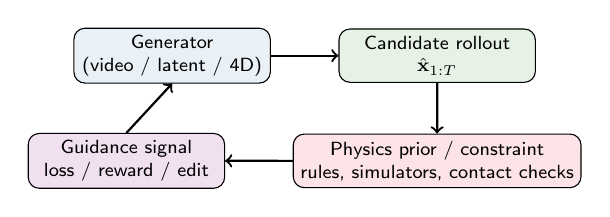
\begin{tikzpicture}[
        scale=0.86, transform shape,
        font=\sffamily\footnotesize,
        block/.style={rectangle, rounded corners, draw, fill=#1!12, inner sep=3pt, align=center, minimum width=2.9cm},
        arrow/.style={->, thick}
    ]
        \node[block=qubitblue] (gen) {Generator\\(video / latent / 4D)};
        \node[block=aigreen, right=1.0cm of gen] (outp) {Candidate rollout\\$\hat{\mathbf{x}}_{1:T}$};
        \draw[arrow] (gen) -- (outp);

        \node[block=controlred, below=0.75cm of outp, minimum width=3.3cm] (phys) {Physics prior / constraint\\rules, simulators, contact checks};
        \draw[arrow] (outp) -- (phys);

        \node[block=quantumpurple, left=1.0cm of phys] (guide) {Guidance signal\\loss / reward / edit};
        \draw[arrow] (phys) -- (guide);
        \draw[arrow] (guide.north) -- (gen.south);
    \end{tikzpicture}
    \caption{Constraint-in-the-loop patterns for physics-aware generation. The ``physics'' component can be a hard constraint, a soft loss, a simulator, or a learned discriminator; the key is that it provides a testable signal tied to dynamics rather than appearance alone \cite{zhang2025think,romero2025learning,zhang2024physdreamer}.}
    \label{fig:physics-schematic}
\end{figure}

\subsection{Interaction and diagnostics}
Interaction-focused methods can couple generation to 3D object representations, enabling ``what-if'' interventions and object-centric control \cite{zhang2024physdreamer}.
Domain-grounded world models (e.g., driving) further provide structured state representations (occupancy, geometry priors) that support more explicit physical checks \cite{yang2025geniedrive}.
Recent work also explores interaction-heavy human-object and human-to-robot settings, where plausibility can be tested by downstream physical feasibility of inferred actions \cite{zhang2025vhoi,ni2025from,ci2025h2r}.

Because physics failures are often subtle, we advocate diagnostics that probe invariances and counterfactual consistency rather than relying only on generic video metrics \cite{romero2025learning,zhang2025think}.
Table~\ref{tab:physics-checklist} lists practical checks that can be adapted to different domains.

\begin{table}[t]
    \centering
    \renewcommand{\arraystretch}{1.05}
    \setlength{\tabcolsep}{4pt}
    \begin{tabular}{p{1.65cm} p{5.6cm}}
        \toprule
        Check & What to test (examples) \\
        \midrule
        Contact & collisions, sliding vs sticking, interpenetration frequency \\
        Forces & gravity direction consistency; acceleration plausibility under control \\
        Conservation & momentum and energy trends in simple rigid-body settings (where measurable) \\
        Constraints & joint limits; nonholonomic constraints in locomotion/wheels \\
        Counterf. & change an object or action; verify localized, causal effects \\
        Long horizon & drift accumulation; stability under repeated interventions \\
        \bottomrule
    \end{tabular}
    \caption{Physics/interaction evaluation checklist. These checks are most informative when paired with a domain definition and explicit control inputs \cite{romero2025learning,zhang2025think,yang2025geniedrive}.}
    \label{tab:physics-checklist}
\end{table}

\section{3D/4D-Aware Generation and Rendering}
Many ``world simulator'' use cases require more than pixel realism: they require a \emph{scene representation} that can be queried, edited, and rendered under viewpoint changes.
This motivates 3D/4D-aware generators that either (i) produce an explicit 3D/4D representation and render video from it, or (ii) use 3D/4D priors to stabilize video generation and control \cite{mildenhall2020nerf,kerbl20233d,wu20234d,gu2025diffusion}.

\subsection{Representations and rendering tradeoffs}
Neural radiance fields (NeRF) represent scenes implicitly and can achieve high fidelity, but typically require costly rendering and optimization \cite{mildenhall2020nerf,pumarola2020d}.
3D Gaussian splatting (3DGS) represents scenes with explicit primitives that enable real-time rendering, at the cost of different regularization and optimization challenges \cite{kerbl20233d}.
4D Gaussian splatting (4DGS) extends this to time-varying scenes, adding temporal regularization and motion modeling challenges \cite{wu20234d}.
Some recent formulations explicitly model 4D Gaussians as a learned dynamical system, strengthening the link between representation learning and motion modeling \cite{asiimwe20254d}.
Figure~\ref{fig:nerf-gs} summarizes the trade space.

\begin{figure}[t]
    \centering
    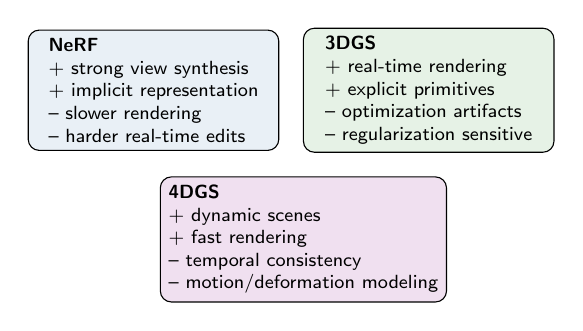
\begin{tikzpicture}[
        scale=0.86, transform shape,
        font=\sffamily\footnotesize,
        card/.style={rectangle, rounded corners, draw, fill=#1!12, inner sep=3.5pt, align=left, minimum width=3.7cm},
    ]
        \node[card=qubitblue] (nerf) {\textbf{NeRF}\\
        + strong view synthesis\\
        + implicit representation\\
        -- slower rendering\\
        -- harder real-time edits};
        \node[card=aigreen, right=0.35cm of nerf] (gs) {\textbf{3DGS}\\
        + real-time rendering\\
        + explicit primitives\\
        -- optimization artifacts\\
        -- regularization sensitive};
        \node[card=quantumpurple, below=0.35cm of gs, xshift=-1.85cm] (4dgs) {\textbf{4DGS}\\
        + dynamic scenes\\
        + fast rendering\\
        -- temporal consistency\\
        -- motion/deformation modeling};
    \end{tikzpicture}
    \caption{Representation tradeoffs for view synthesis and rendering. 4DGS inherits 3DGS speed but must additionally stabilize dynamics over time \cite{mildenhall2020nerf,kerbl20233d,wu20234d,pumarola2020d}.}
    \label{fig:nerf-gs}
\end{figure}

\subsection{From text or video to 4D scenes}
Text-to-3D pipelines often use a strong 2D generator as a prior to optimize a 3D representation (e.g., DreamFusion) \cite{poole2022dreamfusion}.
Gaussian-based pipelines can reduce optimization cost and enable fast rendering, motivating generative 3D and 4D Gaussians \cite{tang2023dreamgaussian,ren2023dreamgaussian4d}.
Text-to-4D Gaussian methods incorporate explicit temporal modeling and alignment strategies to reduce prompt drift and temporal artifacts \cite{ling2023align,miao2024pla4d,deng2025stp4d}.
When the input is video, learned transformers over Gaussian primitives can model dynamics directly from monocular sequences \cite{xu20254dgt}.
Diffusion models can also be trained directly for 3D/4D view synthesis, providing another route to multi-view consistency \cite{fan2025omniview}.
Table~\ref{tab:4d-methods} summarizes representative 3D/4D-aware pipelines and where they sit on the generation--reconstruction spectrum.
Figure~\ref{fig:text-to-4d} highlights common pipeline components.

\begin{table*}[t]
    \centering
    \renewcommand{\arraystretch}{1.05}
    \setlength{\tabcolsep}{4pt}
    \begin{tabular}{p{2.6cm} p{2.6cm} p{3.8cm} p{6.6cm}}
        \toprule
        Method & Input $\rightarrow$ output & Consistency mechanism & Notes \\
        \midrule
        DreamFusion \cite{poole2022dreamfusion} & text $\rightarrow$ NeRF & rendering-loop optimization (SDS) & Strong 2D prior; slower optimization; view consistency emerges from 3D rendering. \\
        DreamGaussian \cite{tang2023dreamgaussian} & text $\rightarrow$ 3DGS & generative Gaussian pipeline & Faster than NeRF optimization; output is explicit primitives for real-time rendering. \\
        DreamGaussian4D \cite{ren2023dreamgaussian4d} & text $\rightarrow$ 4DGS & temporal regularization + generative priors & Dynamic extension; must stabilize motion/deformation and appearance over time. \\
        Align Your Gaussians \cite{ling2023align} & text $\rightarrow$ 4DGS & composed diffusion + alignment & Illustrates modular composition; consistency depends on alignment signals and decomposition. \\
        PLA4D \cite{miao2024pla4d} & text $\rightarrow$ 4DGS & pixel-level alignment & Emphasizes alignment to reduce drift; evaluation must probe temporal stability. \\
        STP4D \cite{deng2025stp4d} & text $\rightarrow$ 4DGS & prompt-consistent spatio-temporal modeling & Targets prompt consistency as a first-class objective; useful for long-rollout stress tests. \\
        4DGT \cite{xu20254dgt} & video $\rightarrow$ 4DGS & transformer dynamics over Gaussians & Learns dynamics from monocular video; connects to spacetime transformers. \\
        OmniView \cite{fan2025omniview} & views $\rightarrow$ 3D/4D synthesis & diffusion for multi-view consistency & Alternative route: train diffusion directly for view synthesis; may not output explicit 4D primitives. \\
        SyncTrack4D \cite{lee2025synctrack4d} & multi-video $\rightarrow$ 4DGS & cross-video motion alignment & Highlights synchronization as a prerequisite for multi-video 4D; correspondence understood as a core primitive. \\
        4DGS dynamical system \cite{asiimwe20254d} & 4DGS $\rightarrow$ dynamics & explicit dynamical-system modeling & Shifts focus from reconstruction to dynamics modeling; useful for ``world model'' discussions. \\
        Diffusion as Shader \cite{gu2025diffusion} & controls $\rightarrow$ video & geometry-aware diffusion guidance & Uses 3D-aware signals to control video without full 4D reconstruction. \\
        Reangle-A-Video \cite{jeong2025reangle} & video $\rightarrow$ re-angled video & implicit 4D via translation & Treats viewpoint change as translation; useful for camera-control framing. \\
        \bottomrule
    \end{tabular}
    \caption{Representative 3D/4D-aware pipelines and their consistency mechanisms. Many systems combine learned components with optimization, and evaluation must separate view consistency from appearance realism.}
    \label{tab:4d-methods}
\end{table*}

\begin{figure}[t]
    \centering
    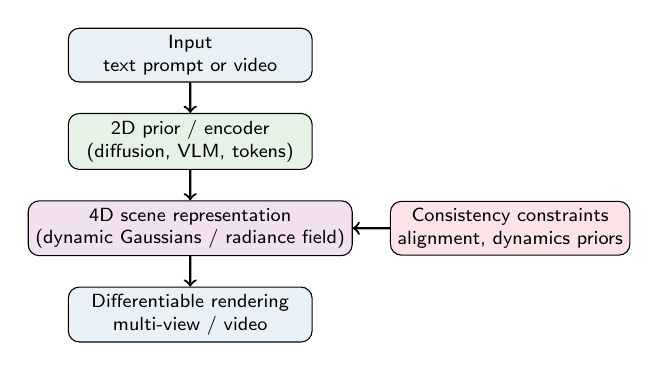
\begin{tikzpicture}[
        scale=0.86, transform shape,
        font=\sffamily\footnotesize,
        block/.style={rectangle, rounded corners, draw, fill=#1!12, inner sep=3pt, align=center, minimum width=3.6cm},
        arrow/.style={->, thick}
    ]
        \node[block=qubitblue] (inp) {Input\\text prompt or video};
        \node[block=aigreen, below=0.45cm of inp] (prior) {2D prior / encoder\\(diffusion, VLM, tokens)};
        \node[block=quantumpurple, below=0.45cm of prior] (rep) {4D scene representation\\(dynamic Gaussians / radiance field)};
        \node[block=qubitblue, below=0.45cm of rep] (rend) {Differentiable rendering\\multi-view / video};
        \node[block=controlred, right=0.55cm of rep, minimum width=2.9cm] (reg) {Consistency constraints\\alignment, dynamics priors};

        \draw[arrow] (inp) -- (prior);
        \draw[arrow] (prior) -- (rep);
        \draw[arrow] (rep) -- (rend);
        \draw[arrow] (reg.west) -- (rep.east);
    \end{tikzpicture}
    \caption{Typical text/video-to-4D pipeline. Methods differ in how much is learned vs optimized, and how temporal consistency is enforced \cite{poole2022dreamfusion,ling2023align,ren2023dreamgaussian4d,deng2025stp4d,xu20254dgt}.}
    \label{fig:text-to-4d}
\end{figure}

\subsection{Alignment and synchronization for multi-video 4D}
When reconstructing or generating a dynamic scene from multiple videos, temporal alignment becomes a first-order problem: inconsistent timing can be misinterpreted as non-rigid deformation or appearance change \cite{lee2025synctrack4d,wu20234d}.
Recent 4D Gaussian methods therefore explicitly address cross-video motion alignment and synchronization, highlighting correspondence as a critical primitive for multi-view dynamic scenes \cite{lee2025synctrack4d,wu20234d}.
For generative 4D pipelines, the same issue appears as prompt-consistency and motion-consistency constraints that must hold across renders and edits \cite{deng2025stp4d,xu20254dgt}.

\subsection{4D-aware video generation and view control}
An alternative to explicit 4D reconstruction is to treat geometry as a \emph{control signal} for video diffusion, which can improve view consistency and enable re-rendering or camera changes \cite{gu2025diffusion,jeong2025reangle,zhang2024recapture}.
This hybrid view blurs generation and rendering: the model may still output pixels, but it is guided by intermediate 3D/4D structure.

\subsection{Integration patterns and failure modes}
4D-aware generation can be viewed as a question of \emph{where} the scene representation sits in the pipeline: as the \emph{primary output} (render-first), as a \emph{latent intermediate} used to guide video generation (generate-first), or as an \emph{editable state} derived from observed video (reconstruct-then-edit) \cite{poole2022dreamfusion,wu20234d,gu2025diffusion,xu20254dgt}.
These choices directly affect what controls are natural to expose.
For example, explicit 4D representations make camera paths and re-rendering ``cheap'' at inference time, while pixel-video generators must internalize camera control as part of the generative process \cite{wu20234d,wang2025bullettime,jeong2025reangle}.

\emph{Render-first} pipelines produce a scene representation (NeRF/3DGS/4DGS or variants) and then render video from it.
They offer a clean interface for view control and can enforce cross-view consistency via the renderer, but they inherit difficult dynamics problems: non-rigid motion, topology changes, and occlusion can be absorbed into the representation in ways that look plausible from some views but fail under viewpoint changes \cite{mildenhall2020nerf,kerbl20233d,wu20234d,asiimwe20254d}.
Multi-video settings amplify this, since time misalignment can masquerade as deformation unless correspondence and synchronization are handled explicitly \cite{lee2025synctrack4d}.

\emph{Generate-first} pipelines keep the output as pixels (or latents) but introduce geometry as a control channel (e.g., depth/pose/camera) or as an intermediate warping prior.
This leverages strong video priors and can support editing and camera changes, but it does not automatically guarantee a consistent underlying scene; geometry may serve as a soft guide that competes with appearance priors and text alignment \cite{gu2025diffusion,zhang2024recapture,jeong2025reangle,kong2025worldwarp}.
In long-horizon generation, this can surface as a mismatch between apparent camera motion and object permanence, especially when occlusions or disocclusions require the model to ``invent'' unseen content \cite{li2024enhancing,zhang2025endless}.

\emph{Reconstruct-then-edit} pipelines infer a 4D representation from video, edit it (or condition generation on it), and render back out.
This supports representation-level constraints (e.g., temporal regularizers) and can make edits more consistent across frames and viewpoints, but it raises new evaluation questions: whether improvements reflect better geometry, better rendering, or simply stronger priors in the editing module \cite{xu20254dgt,zhao2025rdsplat}.
Across these patterns, common failure modes include temporal jitter in geometry, ``floaters'' and ghosting artifacts, prompt drift across time, and fragile edit propagation under viewpoint changes \cite{wu20234d,deng2025stp4d,xu20254dgt}.

Table~\ref{tab:4d-integration} summarizes these integration patterns and the kinds of controls and tests they suggest.

\begin{table}[t]
    \centering
    \renewcommand{\arraystretch}{1.05}
    \setlength{\tabcolsep}{4pt}
    \begin{tabular}{p{1.55cm} p{5.7cm}}
        \toprule
        Pattern & Implications (controls, tests, typical failure modes) \\
        \midrule
        Render-first & Camera/view control at render time; evaluate cross-view stability and time alignment; failures often appear under novel views (jitter, deformation ambiguity) \cite{wu20234d,lee2025synctrack4d}. \\
        Generate-first & Geometry as a soft guide/control; evaluate control adherence vs fidelity tradeoffs and long-horizon occlusion handling; failures include scene inconsistency under edits/view changes \cite{gu2025diffusion,jeong2025reangle}. \\
        Reconstruct-edit & Representation becomes editable state; evaluate whether edits preserve geometry and timing; failures include prior-dominated ``improvements'' that do not generalize \cite{xu20254dgt,zhao2025rdsplat}. \\
        \bottomrule
    \end{tabular}
    \caption{Integration patterns between video generators and 4D scene representations. The pattern suggests which control surfaces are natural and which stress tests are most diagnostic.}
    \label{tab:4d-integration}
\end{table}

\section{Evaluation and Benchmarks}
Evaluation is the hinge between ``impressive demos'' and reproducible scientific progress \cite{unterthiner2018towards,huang2023vbench}.
For spatiotemporal generators, we recommend reporting results along multiple axes: perceptual fidelity, temporal coherence, controllability under structured constraints, and (when applicable) 3D/4D consistency.
No single metric captures these dimensions, and many popular metrics are sensitive to protocol details \cite{unterthiner2018towards,huang2023vbench}.

\subsection{Metrics and what they actually measure}
Distributional metrics such as Fr\'echet Video Distance (FVD) capture some aspects of realism and temporal statistics, but can miss failure modes that humans perceive strongly (identity drift, object persistence, physical implausibility) \cite{unterthiner2018towards}.
Benchmark suites such as VBench aim to cover multiple aspects, but remain constrained by choice of prompts, reference models, and automated proxies \cite{huang2023vbench}.
Targeted benchmarks (e.g., compositional prompts) can reveal systematic generalization gaps that are hidden by aggregate metrics \cite{sun2024t2v}.
More recent work explores reasoning-based evaluation that attempts to align automated judgments with human preferences, at the cost of additional model and prompt dependence \cite{mou2025gradeo,chen2025tivibench}.
As models expand beyond silent video toward audio-visual generation, benchmarks and unified evaluation protocols are emerging for the joint modality \cite{hua2025vabench,cao2025t2av}.

\subsection{Benchmark-to-axis mapping}
Table~\ref{tab:benchmarks} summarizes a small set of widely cited benchmarks and how they map onto the evaluation axes we use throughout the review.
The intended use is to encourage \emph{coverage}: pairing a global metric with targeted tests for coherence, control, and (when relevant) physics or 4D consistency \cite{romero2025learning,zhang2025think,xu20254dgt}.

\begin{table}[t]
    \centering
    \renewcommand{\arraystretch}{1.05}
    \setlength{\tabcolsep}{4pt}
    \begin{tabular}{p{1.85cm} p{5.4cm}}
        \toprule
        Benchmark / metric & Coverage (typical) \\
        \midrule
        FVD & Distributional realism + temporal statistics; weak on fine-grained control and physics \cite{unterthiner2018towards} \\
        VBench & Multi-axis suite for video generators; combines automated proxies and structured tests \cite{huang2023vbench} \\
        T2V-CompBench & Compositional prompt following; probes binding and attribute/object consistency \cite{sun2024t2v} \\
        TiViBench & ``Think-in-video'' reasoning/consistency probes; beyond short-clip fidelity \cite{chen2025tivibench} \\
        Physics tests & Contact/collision and dynamics plausibility (domain-specific) \cite{romero2025learning,zhang2025think} \\
        4D tests & View consistency and temporal stability in dynamic scenes \cite{wu20234d,xu20254dgt} \\
        \bottomrule
    \end{tabular}
    \caption{Benchmarks and metrics mapped to evaluation axes. Coverage varies by protocol; ``physics'' and ``4D'' tests are typically domain- and representation-dependent.}
    \label{tab:benchmarks}
\end{table}

\subsection{Stress tests: long-horizon and intervention consistency}
Aggregate scores can hide long-tail failures that matter for downstream use: identity drift that appears only after many seconds, camera-control artifacts that emerge under large motion, or physics violations that occur only under specific interactions.
We therefore recommend reporting \emph{stress tests} that scale duration and systematically vary control inputs, rather than relying only on average-case prompt suites \cite{huang2023vbench,sun2024t2v,li2024enhancing}.

Stress tests are most informative when framed as controllability problems: specify an input constraint (trajectory, camera path, interaction, or edit), define a measurable success criterion, and report failure rates across a prompt set and multiple seeds \cite{wang2023motionctrl,qiu2024freetraj,romero2025learning}.
For 4D outputs, stress tests should include viewpoint changes and cross-view temporal stability (e.g., camera loops and repeated re-rendering), since these directly probe whether a representation behaves like a stable dynamic scene rather than a collection of per-view hallucinations \cite{wu20234d,xu20254dgt,lee2025synctrack4d}.
Table~\ref{tab:stress-tests} summarizes a few actionable templates.

\begin{table*}[t]
    \centering
    \renewcommand{\arraystretch}{1.05}
    \setlength{\tabcolsep}{4pt}
    \begin{tabular}{p{1.55cm} p{4.25cm} p{5.15cm} p{6.05cm}}
        \toprule
        Axis & Stress test (examples) & What to measure & Common pitfalls \\
        \midrule
        Duration & increase length; vary window stride/overlap & drift rate; reappearance stability; failure counts vs time & reporting only best segments; hidden post-processing for long clips \cite{li2024enhancing} \\
        Coherence & occlusion/reappearance; multi-shot continuity & identity embedding stability; track fragmentation; flicker indicators & biased prompts that avoid occlusion; evaluating only per-frame realism \cite{huang2023vbench} \\
        Control & trajectories, keyframes, and camera paths & path adherence; target localization; camera smoothness under constraints & underspecified depth/occlusion; trading fidelity for compliance without reporting \cite{wang2023motionctrl,qiu2024freetraj} \\
        Editing & local edit at time $t$ (region/instruction) & edit localization; temporal propagation; boundary flicker & leaking edits globally; temporal seams at edit boundaries \cite{liu2023video,zhang2025region} \\
        Physics & contact/collision and counterfactual actions & penetration frequency; causal effect localization; stability under interventions & ``physics'' judged by appearance only; unclear domain definition \cite{romero2025learning,zhang2025think} \\
        4D view & camera loops; render novel views over time & view-consistency; temporal jitter in geometry; re-render stability & mixing renderer settings; measuring only photometric similarity \cite{wu20234d,xu20254dgt} \\
        Multi-video & cross-video synchronization / alignment & timing error; correspondence consistency across views & conflating mis-sync with non-rigid motion; unclear alignment method \cite{lee2025synctrack4d} \\
        \bottomrule
    \end{tabular}
    \caption{Stress-test templates for spatiotemporal generators. The goal is coverage and transparency: define constraints, report measurable success criteria and failure rates, and separate rendering settings from model behavior \cite{huang2023vbench,li2024enhancing,wu20234d}.}
    \label{tab:stress-tests}
\end{table*}

\subsection{Geometry-aware evaluation for 4D outputs}
For explicit 4D representations, evaluation should separate (i) appearance realism under a fixed renderer from (ii) geometric and temporal stability of the underlying scene.
Novel-view metrics (e.g., photometric similarity under held-out views) can be informative, but dynamic scenes introduce alignment and correspondence ambiguities that can dominate results if left underspecified \cite{mildenhall2020nerf,wu20234d,xu20254dgt}.
When multiple videos or viewpoints are involved, time synchronization is part of the method and should be evaluated and reported explicitly \cite{lee2025synctrack4d}.

We recommend reporting a minimal set of 4D-specific protocol details and checks, summarized in Table~\ref{tab:4d-eval-checklist}, alongside the general protocol hygiene guidance in this section.

\begin{table}[t]
    \centering
    \renewcommand{\arraystretch}{1.05}
    \setlength{\tabcolsep}{4pt}
    \begin{tabular}{p{1.55cm} p{5.7cm}}
        \toprule
        Item & What to report / test (examples) \\
        \midrule
        Rep. & NeRF vs 3DGS vs 4DGS; deformation model; renderer settings \cite{mildenhall2020nerf,kerbl20233d,wu20234d} \\
        Views & camera trajectories; view split (train/test); motion distribution \\
        Align. & time sync / correspondence method; failure cases and timing error \cite{lee2025synctrack4d} \\
        Metrics & appearance (PSNR/SSIM/LPIPS); geometry (depth/point error); motion stability (track jitter) \\
        Control & view changes, re-render loops, and edit propagation under constraints \cite{xu20254dgt} \\
        Artifacts & ghosting/floaters; temporal jitter; deformation ambiguity \cite{wu20234d} \\
        \bottomrule
    \end{tabular}
    \caption{A minimal 4D evaluation checklist. The aim is to make view-consistency and temporal stability testable and comparable across pipelines.}
    \label{tab:4d-eval-checklist}
\end{table}

\subsection{Human evaluation and preference protocols}
Human studies remain the most direct way to assess semantic alignment, narrative coherence, and fine-grained artifacts that escape automated metrics.
Human evaluation is a protocol design problem: prompt selection, rater training, pairwise vs absolute scoring, and clip length can substantially change conclusions \cite{huang2023vbench,mou2025gradeo}.
We recommend reporting at least: the full prompt set, the sampling settings, the rater pool definition, and inter-rater agreement (when feasible), and using pairwise comparisons for subtle preferences \cite{huang2023vbench}.
When using vision-language model (VLM) or large language model (LLM) judges, treat the judge as part of the benchmark and report prompts and model versions explicitly \cite{mou2025gradeo,chen2025tivibench}.

\subsection{Protocol and reporting hygiene}
We recommend reporting prompt sets, sampling details, and any post-processing used for long videos, since these choices can dominate the observed failure modes \cite{li2024enhancing}.
For closed systems, the most robust comparisons are those grounded in official documentation and explicitly scoped claims, rather than speculative reconstructions of training data or compute \cite{openai2024sorasystemcard,googlecloud2025veomodelapi}.
Figure~\ref{fig:eval-flow} illustrates a protocol that separates generation, control stress-tests, and evaluation.

\begin{figure}[t]
    \centering
    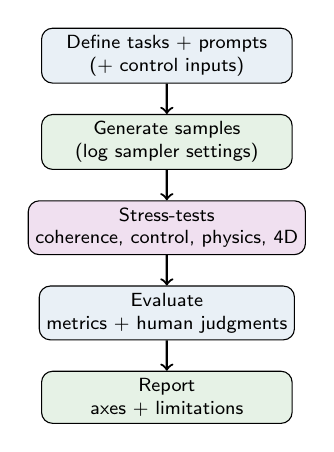
\begin{tikzpicture}[
        scale=0.86, transform shape,
        font=\sffamily\footnotesize,
        step/.style={rectangle, rounded corners, draw, fill=#1!12, inner sep=3pt, align=center, minimum width=3.7cm},
        arrow/.style={->, thick}
    ]
        \node[step=qubitblue] (s1) {Define tasks + prompts\\(+ control inputs)};
        \node[step=aigreen, below=0.45cm of s1] (s2) {Generate samples\\(log sampler settings)};
        \node[step=quantumpurple, below=0.45cm of s2] (s3) {Stress-tests\\coherence, control, physics, 4D};
        \node[step=qubitblue, below=0.45cm of s3] (s4) {Evaluate\\metrics + human judgments};
        \node[step=aigreen, below=0.45cm of s4] (s5) {Report\\axes + limitations};

        \draw[arrow] (s1) -- (s2);
        \draw[arrow] (s2) -- (s3);
        \draw[arrow] (s3) -- (s4);
        \draw[arrow] (s4) -- (s5);
    \end{tikzpicture}
    \caption{Evaluation workflow emphasizing protocol transparency and axis coverage \cite{huang2023vbench,unterthiner2018towards}.}
    \label{fig:eval-flow}
\end{figure}

%%%%%%%%%%%%%%%%%%%%%%%%%%%%%%%%%%%%%%%%%
% SAFETY / PROVENANCE
%%%%%%%%%%%%%%%%%%%%%%%%%%%%%%%%%%%%%%%%%
\section{Safety and Provenance (Optional)}
Frontier video generators raise familiar synthetic-media risks (misinformation, impersonation) and also new risks tied to controllable simulation and interactive rollouts (automated content generation at scale, targeted manipulation).
We keep this section brief and evidence-first: we cite system cards and release notes where available, and treat technical mitigation claims as conditional on explicit threat models \cite{openai2024sorasystemcard,openai2025sora2}.

\subsection{Provenance and attribution}
Provenance mechanisms range from cryptographic content credentials and signing standards to statistical watermarking and detection.
Standards such as C2PA aim to attach verifiable provenance metadata across the content lifecycle \cite{c2pa2025spec}.
Complementary approaches embed watermarks to support detection even when metadata is stripped, though robustness depends on the editing and compression pipeline \cite{fares2025spdmark,jeong2025waterflow,googledeepmind2025synthid}.

\subsection{Detection, robustness, and the attacker model}
Detection is not a solved problem: benchmarks explicitly study de-watermarking, adversarial editing, and human/VLM susceptibility \cite{wang2025robustsora,wang2025video}.
For 3D/4D outputs, provenance extends beyond pixels to scene representations and renderers, motivating representation-level watermarking discussions \cite{zhao2025rdsplat,wu20234d}.
Table~\ref{tab:risk-matrix} summarizes a few concrete risk--mitigation levers and the kinds of evidence we rely on.

\begin{table}[t]
    \centering
    \renewcommand{\arraystretch}{1.05}
    \setlength{\tabcolsep}{4pt}
    \begin{tabular}{p{1.55cm} p{2.35cm} p{3.35cm}}
        \toprule
        Risk & Example failure mode & Mitigation levers (evidence-bounded) \\
        \midrule
        Misuse & misinformation / impersonation & access controls + safety policies; provenance standards; watermarking/detection \cite{openai2024sorasystemcard,c2pa2025spec,fares2025spdmark} \\
        Privacy & training data leakage; face/voice misuse & dataset governance; safety filters; evaluation + red teaming \cite{openai2024sorasystemcard} \\
        IP & copyrighted content replication & provenance metadata; licensing-aware training; auditing \cite{c2pa2025spec} \\
        Detection & de-watermarking / editing attacks & robustness benchmarks; temporal watermark designs; attacker-model clarity \cite{wang2025robustsora,jeong2025waterflow} \\
        3D/4D & re-rendering without attribution & representation-level provenance; renderer-integrated checks \cite{zhao2025rdsplat,wu20234d} \\
        \bottomrule
    \end{tabular}
    \caption{Risk--mitigation matrix for generative video and 4D content. Mitigations are conditional on threat model and deployment constraints; we avoid claiming universal robustness.}
    \label{tab:risk-matrix}
\end{table}

%%%%%%%%%%%%%%%%%%%%%%%%%%%%%%%%%%%%%%%%%
% OPEN CHALLENGES + CONCLUSION
%%%%%%%%%%%%%%%%%%%%%%%%%%%%%%%%%%%%%%%%%
\section{Open Problems and Conclusion}
Despite rapid progress, several open problems remain central for turning video generators into reliable spatiotemporal engines.

\subsection{Open problems}
\begin{itemize}[leftmargin=*]
    \item \textbf{Long-horizon state and memory}: stabilizing identity and scene layout over long rollouts without collapsing diversity remains difficult, and often relies on inference-time heuristics \cite{bartal2024lumiere,li2024enhancing}.
    \item \textbf{Controllability vs generalization}: stronger control signals can improve reliability but may overconstrain the generator or reduce robustness to noisy constraints \cite{wang2023motionctrl,qiu2024freetraj,wang2025bullettime}.
    \item \textbf{Physics and interaction}: adding explicit constraints helps in targeted settings, but general physical plausibility across domains is far from solved \cite{zhang2025think,romero2025learning,yang2025geniedrive}.
    \item \textbf{4D consistency and editability}: dynamic scene representations enable fast rendering and view control, but introduce new failure modes (temporal drift, deformation ambiguity, attribution under re-rendering) \cite{wu20234d,xu20254dgt,zhao2025rdsplat}.
    \item \textbf{Evaluation robustness}: benchmark scores can be fragile to protocol choices; multi-axis evaluation and transparent reporting are necessary for scientific comparability \cite{unterthiner2018towards,huang2023vbench,mou2025gradeo}.
\end{itemize}

\subsection{Conclusion}
Spatiotemporal generative models are converging toward systems that can generate, edit, and (in some cases) simulate dynamic scenes under explicit controls.
A unifying view is to treat ``world simulator'' capability as a spectrum that depends on controllability, temporal/physical consistency, and evaluation hygiene, not just visual fidelity \cite{openai2024worldsimulators,bruce2024genie}.
Progress will likely come from tighter coupling between objectives (diffusion/flow/AR), scene representations (video vs 4D), and evaluation protocols that stress-test coherence, physics, and provenance in realistic deployment settings \cite{lipman2022flow,wu20234d,huang2023vbench}.

%%%%%%%%%%%%%%%%%%%%%%%%%%%%%%%%%%%%%%%%%
% BIBLIOGRAPHY
%%%%%%%%%%%%%%%%%%%%%%%%%%%%%%%%%%%%%%%%%
\clearpage
\bibliographystyle{ieeetr}  
\bibliography{ref} % References are in ref.bib

\end{document} 
